\pdfobjcompresslevel 0
\documentclass[a4paper, 12pt, twoside, openright]{article}

% !TeX root = thesis.tex

%% Reglages des packages %%   
\usepackage[sfdefault]{AlegreyaSans}
\renewcommand*\oldstylenums[1]{{\AlegreyaSansOsF #1}}

\usepackage{dsfont}
\usepackage[utf8]{inputenc}
\usepackage{lmodern}
\usepackage[greek,french]{babel}
\usepackage{enumitem}
\usepackage{amssymb, amsmath, amsfonts, amsthm,mathrsfs}

%--------------------------sur la bio + hyperref
\usepackage[pdfa]{hyperref}
\usepackage{bookmark}

\usepackage[dvipsname,table,xcdraws]{xcolor}

\usepackage[inner=2cm,outer=2cm, bottom=2cm, top=2cm, headheight=15pt]{geometry}

% To create effect on chapter title
\usepackage[explicit, noindentafter]{titlesec}

% Better reference
\usepackage{cleveref}


% package for spacing between lines
\usepackage{setspace}

% package for indentation
\usepackage{indentfirst}

%BUG PACKAGE TITLESEC CORRECTIF
%https://tex.stackexchange.com/questions/299969/titlesec-loss-of-section-numbering-with-the-new-update-2016-03-15
\usepackage{etoolbox}
\makeatletter
\patchcmd{\ttlh@hang}{\parindent\z@}{\parindent\z@\leavevmode}{}{}
\patchcmd{\ttlh@hang}{\noindent}{}{}{}
\makeatother

% Package de mise en page headers
\usepackage{fancyhdr}

% Package pour l'utilisation de sous figures
\usepackage{subcaption}

% TikZ packages
\usepackage{tikz}
\usepackage{pgfplots, pgfplotstable, pgffor}
\usetikzlibrary{arrows}
\usetikzlibrary{shapes}
\usetikzlibrary{positioning}


%les boites
	\usepackage[tikz]{bclogo}
	\usepackage{tikz,tkz-tab}
	\usepackage{pack/boiberne}
	

%Interdire les césures
\usepackage[none]{hyphenat}



%% Credidentials

\makeatletter
\title{Modélisation et étude du métabolisme énergétique cérébral. Applications à
l'imagerie des gliomes diffus de bas grade.}\let\Title\@title
\author{Angélique PERRILLAT-MERCEROT}   \let\Author\@author
\date{22 octobre 2019}        \let\DateSoutenance\@date
\makeatother
% Define my own latex command

%%% Fonts
\newcommand*{\myfont}{\fontfamily{cmr}\selectfont}
\newenvironment{myFont}{\myfont}{\par}
\newenvironment{myCustomFont}{\AlegreyaSans}{}

%%%% Colors
\definecolor{MagSombre}{rgb}{0.5,0.09,0.09}
\definecolor{green_forest}{RGB}{34,139,34}
\definecolor{qqzzqq}{rgb}{0,0.6,0}
\definecolor{ffqqtt}{rgb}{1,0,0.2}
\definecolor{ududff}{rgb}{0.30196078431372547,0.30196078431372547,1}

\definecolor{gris_up}{RGB}{235,235,235}
\definecolor{brun_up}{RGB}{155,137,118}
\definecolor{rouge_up}{RGB}{164,16,42}

\definecolor{vert_lma}{RGB}{1,160,138}
\definecolor{vertf_lma}{RGB}{0,95,80}
\definecolor{bleu_lma}{RGB}{46,69,145}

\definecolor{brun_down}{RGB}{125,109,91}

% Notes in the document
\newcommand\mynotes[1]{\begin{center}
	\vspace{7mm}\textit{\textcolor{rouge_up}{#1}}\vspace{7mm}\end{center}}

%%% Numbering
\setcounter{secnumdepth}{3}

%%% Define a new line spacing
\linespread{1.15}

%%% Config fancyhdr
\pagestyle{fancy}
\fancyhead{}
\fancyfoot{}

\renewcommand{\chaptermark}[1]
	{\markboth{\chaptername ~ \thechapter\ --- #1}{}}
	\renewcommand{\sectionmark}[1]%
	{\markright{\thesection.\ #1}}
\renewcommand{\sectionmark}[1]{\markright{#1}}
\fancyhf{}
	\fancyhead[RO,LE]{\myCustomFont{ \thepage}}
	%\fancyhead[LE]{\myCustomFont{ \leftmark}}
	%\fancyhead[RO]{\myCustomFont{ \rightmark}}
	%\fancyfoot[C]{}
	\renewcommand{\headrule}{\color{gris_up}{\rule{\textwidth}{0.5mm}}}
%	\renewcommand{\headrulewidth}{0.5pt}
%\newcommand{\startChapter}{\vspace{-1.5cm}\minitoc \pagestyle{fancy}}

\fancypagestyle{plain}{%
\fancyfoot[C]{\copyright \\ Page \thepage}
\renewcommand{\headrule}{\color{gris_up}{\rule{\textwidth}{0.5mm}}}
%\renewcommand{\headrulewidth}{0.5pt}
}

%%% Change paragraph appearence        
\titleformat{\paragraph}
{}
{}
{0pt}
{\normalsize\textit{#1}}



%%% Indentation
\titlespacing*{\section}{0pt}{*6}{*2}
\titlespacing*{\subsection}{2em}{*6}{*2}
\titlespacing*{\subsubsection}{4em}{*6}{*2}
\setlength{\parindent}{0.5cm}

%%% raccourcis
\newcommand{\etc}{\textit{etc}}

%%% Hyperref
\hypersetup{
    bookmarks=true,         % show bookmarks bar?
    unicode=false,          % non-Latin characters in Acrobat’s bookmarks
    pdftoolbar=true,        % show Acrobat’s toolbar?
    pdfmenubar=true,        % show Acrobat’s menu?
    pdffitwindow=false,     % window fit to page when opened
    pdfstartview={FitH},    % fits the width of the page to the window
    pdftitle={\Title},    % title
    pdfauthor={\Author},     % author
    pdfsubject={Thèse de modélisation mathématique},   % subject of the document
    pdfcreator={\Author},   % creator of the document
    pdfproducer={\Author}, % producer of the document
    pdfkeywords={Gliome, Modélisation, Cerveau, Substrats, Lactate, Métabolisme énergétique, IRM, SRM, Equations}, % list of keywords
    pdfnewwindow=true,      % links in new PDF window
    colorlinks=true,       % false: boxed links; true: colored links
    linkcolor= MagSombre,
    linkcolor= MagSombre,
    linkbordercolor = white,         
    citecolor= green_forest, % color of links to bibliography
    filecolor=magenta,      % color of file links
    urlcolor=bleu_lma           % color of external links
}


\newenvironment{watermarking}%
{
  % liste des commandes dans l'environnement
  \newcommand{\gf}[1]{\mathbb{F}_{##1}}
  \newcommand{\gftwo}[1]{\mathbb{F}_{2^{##1}}}
  \newcommand{\gfq}[1]{\mathbb{F}_{q^{##1}}}

  \newcommand{\x}{\mathbf{x}}
  \newcommand{\mbf}[1]{\mathbf{##1}}
  \newcommand{\vect}[1]{##1_1, \ldots, ##1_n}
%  \newcommand{\gfq}[1]{\mathbb{F}_{q^{##1}}}
}%
{}

%-------------------------------------------Commandes en supp

%mettre des commentaires
\usepackage{verbatim}



%Pour nettoyer les pages paires entre deux chapitres
\makeatletter
\renewcommand{\cleardoublepage}{%
  \clearpage\fancyhead{}
  \if@twoside
    \ifodd\c@page
      %
    \else
      \hbox{}\newpage
      \if@twocolumn
         \hbox{}\newpage
      \fi
    \fi
  \fi
  
  \fancyhead[RO,LE]{\myCustomFont{ \thepage}}}
\makeatother

%profondeur table des matières
\setcounter{tocdepth}{1}     % Dans la table des matieres 
\setcounter{secnumdepth}{4}  % Avec un numero.


%Mes alinéas
\newcommand{\1}{\displaystyle{\mathds{1}}}
\newcommand{\Li}{\mathscr{L}}
\newcommand{\R}{\mathbb{R}}
\newcommand{\hs}{\hspace{0.02cm}}
\newcommand*{\norm}[1]{\left\lVert#1\right\rVert} % Norme
\newcommand*{\abs}[1]{\left \vert#1 \right \vert} % Valeur absolue
\newenvironment{pushright}{\begin{itemize}\item[\hspace{12pt}]}{\end{itemize}}
\newcommand{\di}{\mbox{d}}
\newcommand{\fat}{$\forall~t \in \mathbb{R}^+$}  
\newcommand{\banana}{{\color{red}\Huge \begin{center}MANQUE IMAGE !\end{center}}}
\newcommand{\bananay}{{\color{red}\Huge \begin{center}MANQUE TEXTE !\end{center}}}


%fonctions avec barre
\newcommand{\fnc}[5]{ \begin{array}{c|ccc} #1: &#2&\longrightarrow &#3\\ &#4&\longmapsto &#5\end{array}} 

%cas
\newcommand{\cas}[4]{#1=\left\{
\begin{array}{rl}
#2 &\text{ si }#3 \\
#4 &\text{ sinon.}
\end{array}
\right.}

%casf
\newcommand{\casf}[3]{\left\{
\begin{array}{rl}
#1 &\text{ si }#2 \\
#3 &\text{ sinon.}
\end{array}
\right.}

%casf2
\newcommand{\casff}[5]{\left\{
\begin{array}{rl}
#1 &\text{ si }#2 \\
#3 &\text{ si }#4 \\
#5 &\text{ sinon.}
\end{array}
\right.}

%cas2
\newcommand{\cass}[5]{#1=\left\{
\begin{array}{rl}
#2 &\text{ si }#3 \\
#4 &\text{ si }#5
\end{array}
\right.}

\newcommand{\fnct}[5]{#1 \left\{
\begin{array}{rl}
#2&\longrightarrow #3\\
#4&\longmapsto  #5
\end{array}
\right.}   


%Diminuer taille titre
\captionsetup{font=small,labelfont={color=MagSombre,bf}}

%%% Create chapter header

\makeatletter
\renewcommand\tableofcontents{%
  \null\hfill\textbf{\Large\color{MagSombre}\contentsname} \hfill\null\par
  \@mkboth{\contentsname}{\contentsname}%
  \@starttoc{toc}%
}
\makeatother


\titleformat{\section}[frame] 
  {\setlength\fboxrule{3pt}\bfseries\fontsize{13.8}{14}\selectfont\color{gris_up}}
  {}{11pt}
  {\color{MagSombre}$\;\;$\thesection .\hskip 0.7em#1}

	
\usepackage[normalem]{ulem}
\usepackage{enumitem}
\usepackage{pdfpages}

\renewcommand{\thefigure}{\textbf{\arabic{section}.\arabic{figure}}}
\renewcommand{\thesubsection}{~~~~~~~~~~~~~~~~\textbf{\arabic{subsection}.}}

\makeatletter
\renewcommand\subsection{\@startsection{subsection}{2}{\z@}%
                                     {-1.5ex\@plus -.3ex \@minus -.2ex}%
                                     {.5ex \@plus .2ex}%
                                     {\normalfont\small\bfseries}}
\makeatother

\DeclareFontFamily{T1}{cmr}{\hyphenchar\font=-1}
\sloppy
\makeatletter
\def\captionoff#1#2{{\def\@captype{#1}#2}}
\makeatother

\makeatletter
\def\clap#1{\hbox to 0pt{\hss #1\hss}}%
\def\ligne#1{%
\hbox to \hsize{%
\vbox{\centering #1}}}%
\def\haut#1#2#3{%
\hbox to \hsize{%
\rlap{\vtop{\raggedright #1}}%
\hss
\clap{\vtop{\centering #2}}%
\hss
\llap{\vtop{\raggedleft #3}}}}%
\def\bas#1#2#3{%
\hbox to \hsize{%
\rlap{\vbox{\raggedright #1}}%
\hss
\clap{\vbox{\centering #2}}%
\hss
\llap{\vbox{\raggedleft #3}}}}%
\def\maketitle{%
\thispagestyle{empty}\vbox to \vsize{%
{\color{gris_up}\hrule height 3pt}
\vspace{1cm}
\begin{flushleft}
\usefont{OT1}{ptm}{m}{n}
\begin{center}
{\huge Candidature au poste de MCF}\\
\textit{Section CNU 25, 26 et 69.}
\end{center}
\end{flushleft}
\vspace{1cm}
{\color{gris_up}\hrule height 3pt}


\vfill

\begin{center}
{\color{brun_up}\Large \textbf{Angélique Perrillat-Mercerot}}\\
Ingénieur de Recherche / Post-doctorante en Mathématiques\\
Qualifiée en sections CNU 26 (mathématiques appliquées), 25 (mathématiques) et 69 (neurosciences),\\
Université de Poitiers, Laboratoire commun I3M (CNRS-UP-CHU-Siemens Healthineers),\\
Laboratoire de Mathématiques et Applications, UMR CNRS 7348  SP2MI, Equipe DACTIM-MIS,\\
Site du Futuroscope - Téléport 2, 11 Boulevard Marie et Pierre Curie, F-86073 Poitiers cedex 9,\\
CHU de Poitiers, 2 Rue de la Milétrie, F-86021 Poitiers,\\
E-mail : angelique.perrillat@math.univ-poitiers.fr\\
Site : \href{https://aperrillat.wixsite.com/sitehttp://texnique.fr/osqa/faq/}{aperrillat.wixsite.com/site}.
\end{center}

\vfill

{\setlength{\baselineskip}{0.3\baselineskip}
\tableofcontents\par}

\vfill
\bas{}{Poitiers, Mars 2020}{}
}%
\cleardoublepage
}
\def\date#1{\def\@date{#1}}
\def\author#1{\def\@author{#1}}
\def\title#1{\def\@title{#1}}
\def\location#1{\def\@location{#1}}
\def\blurb#1{\def\@blurb{#1}}
\date{\today}
\author{}
\title{}
\location{Poitiers}\blurb{}
\makeatother


\begin{document}
\maketitle

%---------------------PARTIE 1----------------------------------


\section{Parcours \& Compétences}

\begin{enumerate}
\item[\color{MagSombre}$\bullet$] \textbf{\color{MagSombre} Résumé du parcours.} Seules les affiliations relatives aux mathématiques sont précisées.
\begin{itemize}
\item[$\triangleright$] \textit{Licence en mathématiques générales et applications, Université de Lyon, 2014.}\\
UEs complémentaires en physique : Electromagnétisme et physique des ondes, Optique et Mécanique des systèmes solides. Options supplémentaires : Italien (Institut culturel italien) et Génétique et Dynamique des Populations (Université Lyon 1, parcours SVT).
\item[$\triangleright$] \textit{Master Maths en Action - Mathématiques pour la biologie et la médecine, Université de Lyon, 2016.}\\
Cours de M1 : Logiciels Scientifiques (Maple, Scilab, Matlab, R), Probabilité, Analyse Appliquée et Equations aux Dérivées Partielles, Systèmes Dynamiques, Séries Chronologiques, Statistiques Paramétriques, Recherche Opérationnelle et Optimisation Discrète, Calcul Scientifique, Anglais et Gestion de projet sous la direction de Simon Masnou (PR, ICJ, Lyon).\\ UE supplémentaire en M1 : Analyse Numérique et Optimisation.\\
Cours de M2 : Analyse Appliquée, Dynamique des populations, Statistique en grande dimension, Dynamique des protéines, Modélisation stochastique et statistique et Stage de recherche sous la codirection de Laurent Pujo-Menjouet (MCF, ICJ, Lyon), Léon Matar Tine (MCF, ICJ, Lyon), Pauline Mazzocco (chercheuse Adocia, Lyon) et Human Rezaei (DR INRA).
\item[$\triangleright$] \textit{Doctorat en mathématiques appliquées, Université de Poitiers, 2019.}\\
Titre : \textit{Modélisation et étude du métabolisme énergétique cérébral. Applications à
l'imagerie des gliomes de bas grade.}\\ 
Directeurs : Alain Miranville (PR, LMA, Poitiers) et Rémy Guillevin (PU-PH radiologie et imagerie médicale).\\ Rapporteurs : Olivier Saut (DR CNRS, Inria BSO) et Jean Noël-Vallée (PU-PH radiologie et imagerie médicale).\\ Examinateurs : Frédérique Clément (DR, Inria Paris), Jacques Demongeot (PU-PH émérite biostatistiques, informatique médicale et technologies de communication), Jean-Pierre Françoise (PR émérite, LJLL, Paris) et Luc Pellerin (PR biochimie et biologie moléculaire).\\ Invités : Nicolas Bourmeyster (PU-PH biochimie et biologie moléculaire) et Anne-Karine Bouzier-Sore (CR CNRS, spécialité biochimie et biologie moléculaire).
\item[$\triangleright$] \textit{Contrat de DCACE puis vacation, Université de Poitiers, 2017-2020.}\\
Vacation de 64h d'enseignement par an détaillée en section \ref{ens}.
\item[$\triangleright$] \textit{Ingénieur de Recherche - Postdoctorat en mathématiques, CHU de Poitiers, en cours.}\\
Thème : \textit{Etude dynamique du métabolisme énergétique cérébral par la modélisation mathématique.}
\end{itemize}
\vspace{0.3cm}
\item[\color{MagSombre} $\bullet$] \textbf{\color{MagSombre} Compétences linguistiques.}
\begin{itemize}
\item[$\triangleright$] Français langue maternelle (C2),
\item[$\triangleright$] Anglais lu, écrit, parlé (C1),\textit{ 790 pts au TOEIC - Jan. 2016 (durant le master),}
\item[$\triangleright$]  Italien lu, écrit, parlé (C1), \textit{CLES B2 - Fev. 2019.}
\end{itemize}
\vspace{0.3cm}
\item[\color{MagSombre} $\bullet$] \textbf{\color{MagSombre} Compétences informatiques.}
\begin{itemize}
\item[$\triangleright$]Logiciels : \LaTeX , Office, Inkscape, Photofiltre.
\item[$\triangleright$]Programmation : Matlab, R, Python, Scilab, Maple.
\end{itemize}
\end{enumerate}

\newpage
\section{Activité d'Enseignement}\label{ens}
\begin{itemize}
\item[\color{MagSombre}$\bullet$] \textbf{\color{MagSombre}Contrat de vacataire (2017-2020).}
\begin{itemize}
\item[$\triangleright$] 28h de colles (examens oraux) en mathématiques pour les L1/L2 Parcours renforcé, Université de Poitiers (2017-2018). Groupes de 6 élèves en binôme. Création de questions de cours et de feuilles d'exercices adaptés pour les différents thèmes et niveaux, correction des copies, retours avec notes et remarques individuelles et collectives pour les professeurs et élèves,
\item[$\triangleright$] 36h (2017-2018) + 64h (2018-2019) de TD en mathématiques générales pour les L1 SVT/BGSTU, Université de Poitiers. Groupes allant de 31 à 42 élèves. Mise en place de sessions d'exercices supplémentaires de type examen blanc ou avec support interactif, 
\item[$\triangleright$] 64h (2019-2020) de TD en calcul matriciel pour les L1 informatique, Université de Poitiers. Groupes allant de 35 à 60 élèves. Mise en place d'interactions pédagogiques entre les élèves d'un même TD et entre plusieurs groupes de TD,
\item[$\triangleright$] Mise à disposition en temps réel de l'avancement, des exercices donnés, d'exercices autres et d'une zone de contact permettant de poser des questions en ligne sur mon site internet. Participation aux tâches annexes : vérification des sujets d'examen, surveillances d'examens, correction des copies, mise à disposition des corrections et explications aux étudiants.
\end{itemize}
\item[\color{MagSombre}$\bullet$] \textbf{\color{MagSombre}Encadrement de stagiaire.} Encadrante principale d'un stagiaire issu du M1 Statistiques et Données du Vivant de Poitiers : Clément Giraud. Stage de 4 mois (avril-aout 2020) sur la thématique : \textit{Analyse multiparamétrique de données métaboliques issues de l'IRM dans l'ischémie-reperfusion cérébrale}. Ce travail, en collaboration avec un interne en médecine et un radiologue, inclut rapport et présentation orale.  
\item[\color{MagSombre}$\bullet$] \textbf{\color{MagSombre}Crédo pour l'enseignement.} Je suis pour un enseignement accessible et personnalisé. Ainsi j'incite fortement mes élèves à s'exprimer au tableau, à l'oral ou lors de rendez-vous mais aussi par mail ou sur mon site internet. Les questions qui y sont posées peuvent être anonymes et je les traite alors en TD pour tout le monde, le cas échéant. Les outils numériques sont au coeur de mon enseignement avec un suivi de l'avancement et des exercices supplémentaires disponibles en ligne en temps réel mais également la mise en place d'exercices types QCM où les élèves répondent en direct et avec un temps limité grâce à leurs téléphones ou ordinateurs.
\item[\color{MagSombre}$\bullet$] \textbf{\color{MagSombre}Activité liée à la Popularisation.}
\begin{itemize}
\item[$\triangleright$] Co-organisation locale du congrès Maths-En-Jeans 2018 à Poitiers. Cogestion des locaux, des repas, des nuitées, des transports et des présentations pour plus de 700 participants sur trois~jours, mars 2018,
\item[$\triangleright$] Perrillat-Mercerot A. \textit{Modélisation et étude du métabolisme énergétique cérébral. Applications à l’imagerie des gliomes diffus de bas grade.} Répétition de soutenance de thèse dans le cadre du printemps de la Recherche à l'Université de Poitiers, mars 2020,
\item[$\triangleright$] Tenu de stands pour des actes annuels de popularisation des mathématiques tout public : fêtes de la science à Poitiers (2017,2018) et nuit des chercheurs au CHU de Poitiers (2018,2019),
\item[$\triangleright$] Interventions dans des écoles et MJC pour la popularisation de la recherche et des mathématiques, des sciences et de la Recherche en milieu scolaire : Femmes \& Sciences (lycéens, Montmorillon (86)), association Nombredor sous la direction de Madalina Petcu (lycéens de Parthenay, en visite d'un site de recherche à Chasseneuil du Poitou (86)), échange en école primaire sous la direction de Coralie Perrillat -Mercerot (élèves en cycle 3, CM1 et CM2, Saint-Agnès (06)), Sciences En Mouvement D'Elles organisé par l'Espace Mendès France (collégiens, Lusignan (86)).
\item[$\triangleright$] Deux publications orientées grand-public :
\begin{itemize}
\item \textit{En tête à tête}, Microscoop : magazine de la délégation CNRS Centre
Limousin Poitou-Charentes, 78(2018), 14-15,
\item  (coécrit avec Paul Dequidt, laboratoire de traitement d'image XLIM), \textit{Des données biologiques aux modèles
et inversement}, Site Image Des Mathématiques, session échos de la Recherche.
\end{itemize}
\end{itemize}
\item[\color{MagSombre}$\bullet$] \textbf{\color{MagSombre}Bénévolat.} 56h de bénévolat, aide en terminal S et préparation au baccalauréat de mathématiques (2018-2019). Suivi personnalisé avec création d'exercices adaptés, de devoirs supplémentaires et mise en place d'exercices type QCM au début de chaque session.
\end{itemize}

\section{Activité Administrative \& Autres Responsabilités Collectives}
\begin{itemize}
\item[\color{MagSombre}$\bullet$] \textbf{\color{MagSombre}Représentante des doctorants} de l'école doctorale (ED) SISMI (ex S2IM) de juil. 2017 à oct. 2019 :
\begin{itemize}
\item[$\triangleright$] Aide à la communication entre l'administration de l'école doctorale et les doctorants, notamment avec la gestion de sondages,
\item[$\triangleright$] Mise en place et coorganisation de séminaires mensuels entre doctorants,
\item[$\triangleright$] Coorganisation de journées pour la vision de l'après-thèse avec intervenants extérieurs,
\item[$\triangleright$] Participation à la commission d'examen des candidats à un doctorat dans l'ED,
\item[$\triangleright$] Mise à disposition d'une page internet contenant les informations principales pour le bon déroulement d'une thèse dans l'ED SISMI en français et en anglais sur mon site internet.
\end{itemize}
\item[\color{MagSombre}$\bullet$] \textbf{\color{MagSombre}Accueil} au sein du Laboratoire de Mathématiques et Applications et pour l'équipe DACTIM-MIS (2017-2020), en particulier présentations pour des délégations de centre de Recherches extérieurs et prise en charge de stagiaires de 3ème dans le cadre de stage d'observation d'une semaine : Alix Renoncourt (février 2018, sous la direction de Morgan Pierre) et Martin Dupin (janvier 2020, sous la direction de Pol Vanhaecke).
\item[\color{MagSombre}$\bullet$] \textbf{\color{MagSombre}Coorganisation d'une conférence interdisciplinaire internationale,} IbOMaN avec Hugo Martin, Alexandre Poulain et Emma Leschiera au laboratoire Jacques-Louis Lions (Paris, Sorbonne université). Cette conférence aura lieu sur deux jours en Juin 2020 avec dix orateurs issus des mathématiques, du numérique, de la biologie et/ou du médical et deux parrains Francis Levi et Jacques Demongeot. Création de dossiers pour la demande de fonds, en particulier lors de l'appel à projet BOUM de la SMAI, recherche et gestion des parrains et des orateurs, cogestion de la communication, des locaux, des repas, des nuitées, des transports et des présentations.
\item[\color{MagSombre}$\bullet$] \textbf{\color{MagSombre}Suivi de formations sur site} pour le bon déroulement de mes activités d'enseignement et d'accueil : Conduite de thèse, Gestion d'équipe, Formation pour l'enseignement, Formation à la pédagogie universitaire \& Formation d'espagnol, Université de Poitiers, Chasseneuil du Poitou.
\end{itemize}

\section{Activité de Recherche}\label{AR}
Mes recherches portent avant tout sur l'analyse et la modélisation de processus biologiques. Elles sont en particulier axées sur l'étude des mécanismes reliés aux neurosciences et aux dynamiques cellulaires : interactions entre cellules ou protéines, flux nutritifs, dynamique tumorale, approche \textit{in vivo}, IRM cérébrale, SRM. Les démarches mathématiques mises en place dans ces recherches sont nombreuses, allant de la description statistique à la modélisation et l'étude de modèles multi-échelle à l'aide d'équations différentielles ordinaires (EDO), d'équations différentielles ordinaires à retard (EDR) et d'équations aux dérivées partielles (EDP).

\begin{itemize}
\item[\color{MagSombre}$\bullet$] \textbf{\color{MagSombre}Stage de 6 mois en M2 sous la codirection de Laurent Pujo-Menjouet, Léon Matar Tine, Pauline Mazzocco et Human Rezaei, Inria de Villeurbanne, (UMR 5208 \& 5534), équipe Dracula, 2016.} Découverte en 1906 par Aloïs Alzheimer, la maladie d'Alzheimer est une infection du cerveau qui entraîne la disparition progressive des neurones. Cependant les mécanismes de cette progression restent encore mal connus. Ainsi, 90\% de ce que nous savons aujourd'hui a été mis en évidence ces 20 dernières années. Aujourd'hui nous avons montré que deux agents sont intimement liés aux symptômes de la maladie, mais dans quelles mesures la protéine prion et le peptide A$\beta$ peuvent-ils être considérés comme responsables \cite{resenberger2011,gimbel2010} ? Ce stage porte sur un modèle d'interaction entre les différents agents en jeu grâce à un modèle de 37 équations (incluant des EDO, des équations à retard et des équations de masse) basées sur les équations de Becker-Döring (voir la Figure \ref{stage}). Nous présentons une étude des équilibres, des simulations et des comparaisons aux résultats biologiques. En particulier une fonction de Lyapunov non triviale est utilisée pour prouver la stabilité globale de l'état d'équilibre préalablement mis en évidence.\\
\textbf{Communications liées }: Un article publié $\left[ \text{C8} \right]$ , une communication orale lors d'un séminaire interne.
 \begin{figure}[!htbp]
\centering
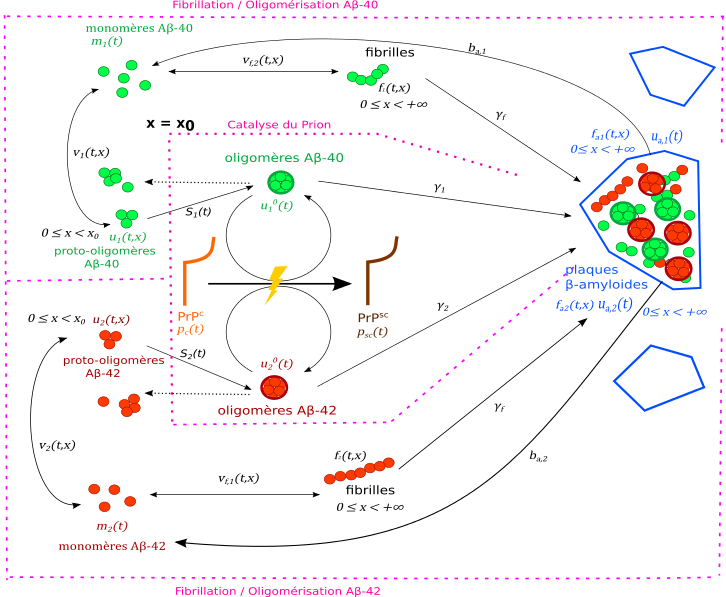
\includegraphics[width=0.6\textwidth]{schem.png}
\caption{Schéma du modèle mis en place lors de mon stage afin d'expliquer l'impact de l'intéraction des différentes protéines A$\beta$ sur la protéine Prion lors de la maladie d'Alzheimer.}\label{stage}
\end{figure}
\newpage
\item[\color{MagSombre}$\bullet$] \textbf{\color{MagSombre}Doctorat sous la codirection d'Alain Miranville et Rémy Guillevin, Université de Poitiers, Laboratoire de Mathématiques et Applications (LMA, UMR 7348), équipe DACTIM-MIS, 2016-2019.}  Tout ce qui vit naît, se nourrit, se reproduit et meurt. Pour le cerveau, la question se complexifie car à la survie des neurones s'ajoute le coût de l'activité cérébrale. La question de la gestion énergétique pour les neurones est particulière car les cellules de notre cerveau évoluent de manière concertée et non par compétition. On sait avec l'imagerie médicale que l'usine neuronale ne fonctionne pas uniquement grâce au glucose ; elle utilise d'autres apports énergétiques tels que le lactate ou le glutamate pour soutenir sa production \cite{pellerin1994}. Lorsqu'une tumeur apparaît, elle change le métabolisme énergétique pour survivre et soutenir sa propre croissance. En particulier, les cellules cancéreuses se fournissent en lactate et choisissent leur substrat préféré en fonction de l'oxygène disponible \cite{romero2016, walenta2016}. La modélisation mathématique des substrats énergétiques est un outil de choix pour décrire et prédire de tels flux. Coupler ces modèles à des données issues de l'IRM et de la SRM permet d'améliorer la prise en charge du patient présentant un gliome. Ma thèse propose l'approche de plusieurs dynamiques en substrat dans le cerveau sain et gliomateux en se basant sur des systèmes d'équations : échanges locaux en lactate (EDO, système lent-rapide), échanges globaux en substrats (EDO), cycle glutamate/glutamine (EDR) et échanges en lactate en dimensions supérieures (EDP). Ces modèles sont expliqués, décrits grâce aux mathématiques et permettent l'élaboration de simulations ajustées selon des données patient ou issues de la littérature. Ainsi mon travail de thèse
s'oriente autour de trois axes principaux,
\begin{itemize}
\item[$\triangleright$]\textit{Axe 1. Synthèse historique de l'apport de la modélisation mathématique dans l'approche des comportements gliomateux}, en particulier pour les échanges énergétiques. Cette partie compose trois des chapitres de ma thèse et permet d'apprécier le positionnement de la problématique des échanges énergétiques dans les enjeux actuels sur la compréhension des mécanismes cérébraux. Les articles $\left[ \text{C3} \right]$ et $\left[ \text{C4} \right]$ sont issus de cet axe.
\item[$\triangleright$]\textit{Axe 2. Modélisations en 1D de flux en substrats énergétiques dans le milieu cérébral}, analyse et simulations. Ces recherches sont en collaboration avec Nicolas Bourmeyster, laboratoire de physiologie cellulaire Signalisation et Transports Ioniques Membranaires (STIM, ERL CNRS 7003). Cette partie constitue quatre de mes chapitres de thèse sur différentes dynamiques modifiées dans les amas tumoraux. En particulier des EDOs et des outils statistiques (tests paramétriques, indices de Sobol) sont utilisés. Le premier modèle étudié décrit les flux de lactate entre une cellule et le sang à travers un monocarboxylate transporter (MCT). Le modèle est donné \textit{in vivo} ce qui nécessite la prise en compte du flux sanguin continu des artères aux veines. Il est composé de termes non linéaires prisés des biologistes. Ce système lent-rapide a été initialement proposé par Agnès Aubert dans sa thèse \cite{Taubert, aubert2005}. Dans cette approche, deux variables sont présentes : la concentration en lactate intracellulaire $u$ et la concentration en lactate du capillaire $v$ (voir Figure \ref{Lac}(a)). \hs Le système suivant propose alors le suivi local des flux de lactate autour de la barrière hémato-encéphalique, \fat ,
\vspace{-0.25cm}
\begin{align*}
{u'}_{\varepsilon}(t) &= J(t,u_{\varepsilon}(t))-T(\frac{u_{\varepsilon}(t)}{k+u_{\varepsilon}(t)}-\frac{v_{\varepsilon}(t)}{k'+v_{\varepsilon}(t)}), \\ 
 \varepsilon {v'}_{\varepsilon}(t) &= F(t)(L-v_{\varepsilon}(t))+T(\frac{u_{\varepsilon}(t)}{k+u_{\varepsilon}(t)}-\frac{v_{\varepsilon}(t)}{k'+v_{\varepsilon}(t)}).
\end{align*}
\vspace{-0.25cm}
On montre en particulier les similarités et les différences de comportement entre le système pour $\varepsilon>0$ et celui pour $\varepsilon=0$ grâce à des outils analytiques et numériques dans une nouvelle approche. Le deuxième modèle étudié propose le suivi de trois types de populations cellulaires : les neurones, les astrocytes et les cellules gliomateuses. Les substrats considérés sont l'oxygène (neuronal, astrocytaire et gliomateux), le glucose (neuronal, astrocytaire et gliomateux) et le lactate (neuronal, astrocytaire et gliomateux). Le lactate et le glucose peuvent se retrouver dans le milieu extracellulaire  alors que lactate, glucose et oxygène peuvent être transportés via le réseau sanguin (voir Figure \ref{Lac}(b)). Glucose et oxygène ou lactate et oxygène sont utilisés ensemble par une population de cellules pour créer de l'énergie. Le glucose peut également être transformé en lactate créant moins d'énergie. Cette énergie est utilisée pour maintenir l'activité cellulaire. De manière innovante, l'énergie consommée définie alors une capacité du milieu pour chaque population. Cette capacité variable en temps est prise en compte dans des équations de Verhultz. On montre en particulier, grâce à ce système de 17 équations, les liens entre flux énergétique et croissance gliomateuse mais également l'avantage donné aux cellules gliomateuses dont les ressources énergétiques sont adaptables.
Dans le troisième modèle étudié, glutamate et glutamine, possèdant un rôle central dans le transport de l'information cérébrale, sont considérés. Dans le cycle formé entre neurones et astrocytes,  seulement 20~\%~-~25~\% du flux en glutamine est nouvellement synthétisé, le reste provient d'un recyclage \cite{hertz2017}. On obtient un système d'EDOs possédant un retard et des termes non linéaires pour rendre compte des échanges entre glutamate neuronal, glutamate extracellulaire, glutamate astrocytaire, glutamine astrocytaire et glutamine neuronale (voir Figure \ref{Lac}(c)). Finalement nous avons les équations aux dérivées ordinaires avec retard suivantes pour $t \in \mathbb{R}^+$, $t\geqslant \tau$,
\vspace{-0.25cm}
\begin{align*}
A_n'(t) &= t_nI_n(t)-f(t)A_n(t)+\beta_1f(t-\tau)A_n(t-\tau),\\
A_e'(t) &=f(t)A_n(t)-f(t-\tau)A_n(t-\tau),\\
A_a'(t) &=\beta_2 f(t-\tau)A_n(t-\tau)-t_aA_a(t),\\
I_a'(t) &= t_aA_a(t)-w\frac{I_a(t)}{I_a(t)+\omega_a}+(1-\beta_1-\beta_2)f(t-\tau)A_n(t-\tau),\\
I_n'(t) &= w\frac{I_a(t)}{I_a(t)+\omega_a}-t_nI_n(t). 
\end{align*}
\vspace{-0.25cm}
Et, en fonction initiale sur $]0,\tau[$ un système équivalent sans les termes retardés. On montre en particulier dans cette étude le bon comportement du système malgré le retard mais également ses réactions en condition pathologique ce qui a ouvert des questionnements biologiques.
Ces trois approches constituent les articles $\left[ \text{C5} \right]$, $\left[ \text{C6} \right]$ et $\left[ \text{C7} \right]$.

\begin{figure}[!htbp]
\centering
\begin{minipage}{0.3\textwidth}
  \centering
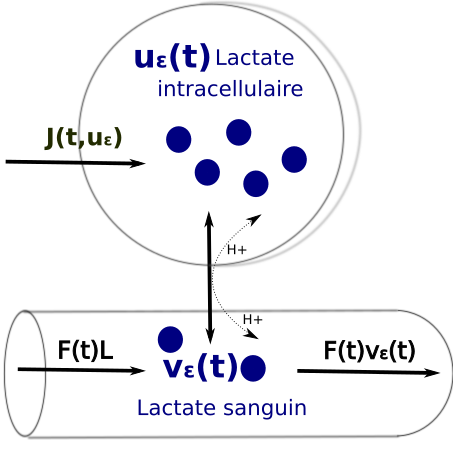
\includegraphics[width=0.8\textwidth]{dessin.png}
\subcaption{Lactate local.}
\end{minipage}
\hspace{-0.5cm}
\begin{minipage}{0.35\textwidth}
  \centering
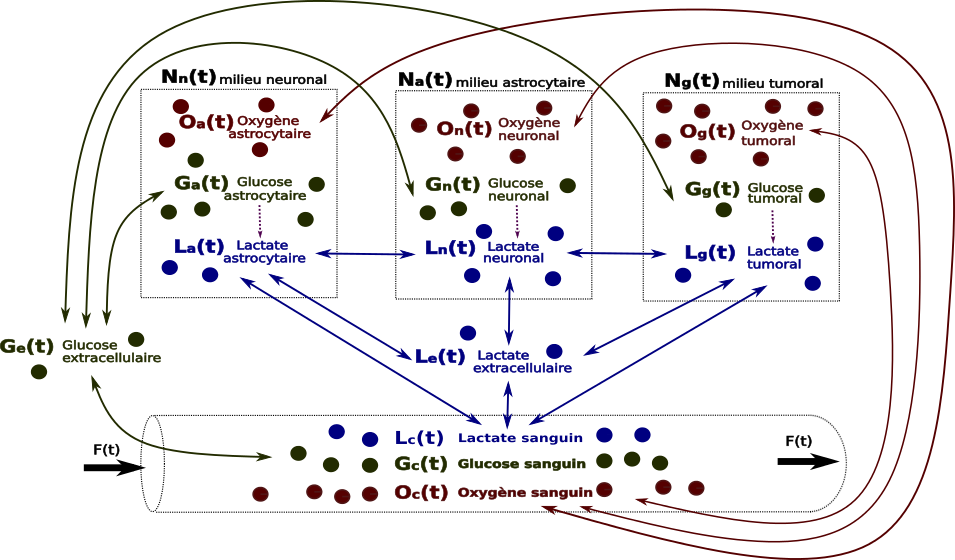
\includegraphics[width=1.05\textwidth]{dessin2.png}
\subcaption{Substrats globaux.}
\end{minipage}
\hspace{0.2cm}
\begin{minipage}{0.3\textwidth}
\centering
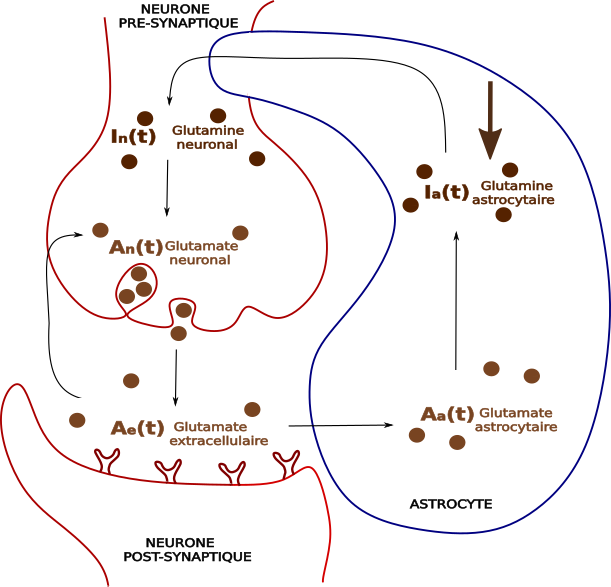
\includegraphics[width=0.8\textwidth]{dessin3.png}
\subcaption{Cycle glutamate.}
\end{minipage}
\caption{Schéma des modèles mis en place dans cet axe pour le suivi des flux énergétiques. (a) Flux lactate locaux, (b) Flux globaux entre astrocytes, neurones et cellules glimateuses, (c) Cycle glutamate-glutamine avec retard. }\label{Lac}
\end{figure}

\newpage
\item[$\triangleright$]\textit{Axe 3. Modélisations en dimension supérieure des échanges en lactate entre neurones et astrocytes}, analyse et simulations. Ces recherches sont en collaboration avec les départements de mathématiques de Milan et de Pavie, en particulier Abramo Agosti, Maurizio Grasselli, Elisabetta Rocca et Pasquale Ciarletta à l'origine des articles \cite{agosti2018,agosti2019}. Cette partie constitue trois de mes chapitres de thèse dans lesquels sont étudiés des systèmes d'EDPs aux conditions de bord complexes pour comprendre les possibilités d'utilisation des mathématiques pour la compréhension des cartes cérébrales issues de la SRM. 
Dans un premier temps nous avons repris le modèle proposé dans $\left[ \text{C7} \right]$ et nous l'avons réécrit comme un modèle de réaction-diffusion couplé à des conditions de bord de type Neumann (voir Figure \ref{Lac2}(a)). Ce système est donné \fat, \begin{gather*}
\frac{\partial u}{\partial t}-D_u \Delta u+\kappa ({u\over {k+u}}-{w\over {k'+w}})
=J, \\
\varepsilon \frac{\partial w}{\partial t}-D_w \Delta w+Fw
+\kappa ({w\over {k'+w}}-{u\over {k+u}})=FL,
\end{gather*}
où $u=u(x,t)$ et $w=w(x,t)$,
que l'on considère sur un domaine régulier borné $\Omega $ de
$\mathbb{R}^N$, $N=1$, $2$ ou $3$,
avec les conditions de bord de type Neumann suivantes,
$$
\frac{\partial u}{\partial \nu}=\frac{\partial w}{\partial \nu}
=0\quad\text{sur }\Gamma ,
$$
En particulier nous avons montré le bon comportement du système d'EDPs qui est assimilable à son homologue d'EDOs, nous avons également proposé des simulations. Dans un second temps, nous avons proposé et étudié un modèle où les échanges en substrat sont possibles uniquement dans certaines zones que l'on nomme interfaces (voir Figure \ref{Lac2}(b) et \ref{Lac2}(c)). Ces considérations donnent lieu à des conditions de bord complexes qui rendent les résultats analytiques plus difficiles à obtenir. Assumant l'existence des solutions, nous avons montré la positivité et l'unicité des solutions et proposé des simulations. Cette étude est toujours en cours. Les articles $\left[ \text{C2} \right]$ (en travail) et $\left[ \text{C9} \right]$ sont issus de cet axe.
\end{itemize}

\begin{figure}[!htbp]
\centering
\begin{minipage}{0.33\textwidth}
  \centering
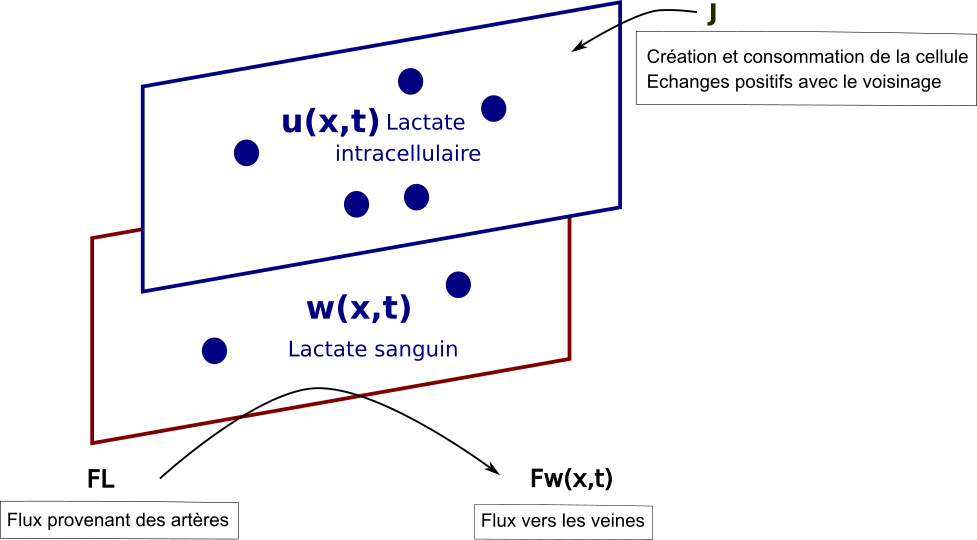
\includegraphics[width=1\textwidth]{dessinD.png}
\subcaption{Réaction-Diffusion.}
\end{minipage}
\begin{minipage}{0.33\textwidth}
  \centering
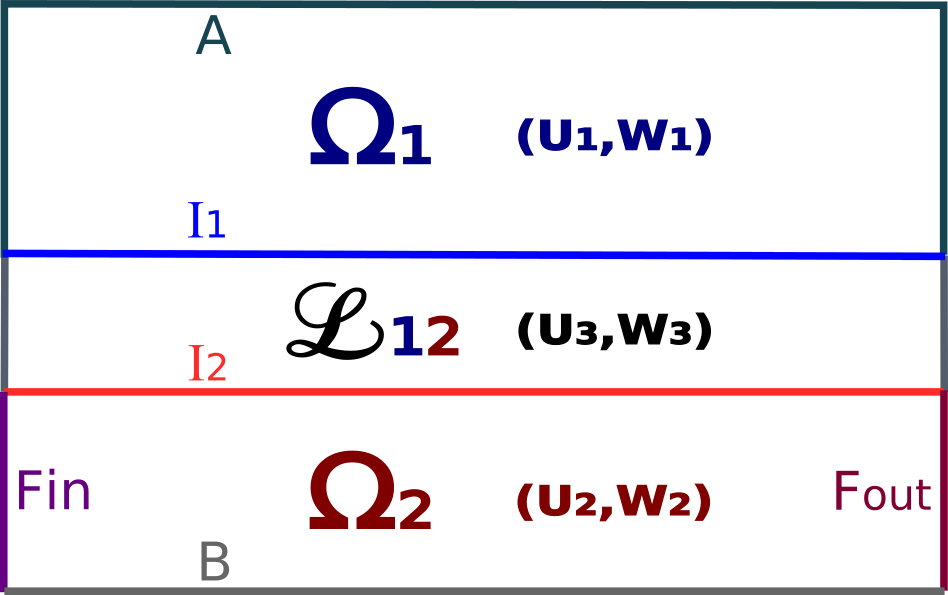
\includegraphics[width=0.9\textwidth]{dessinD2.png}
\subcaption{Schema avec interface.}
\end{minipage}
\begin{minipage}{0.33\textwidth}
\centering
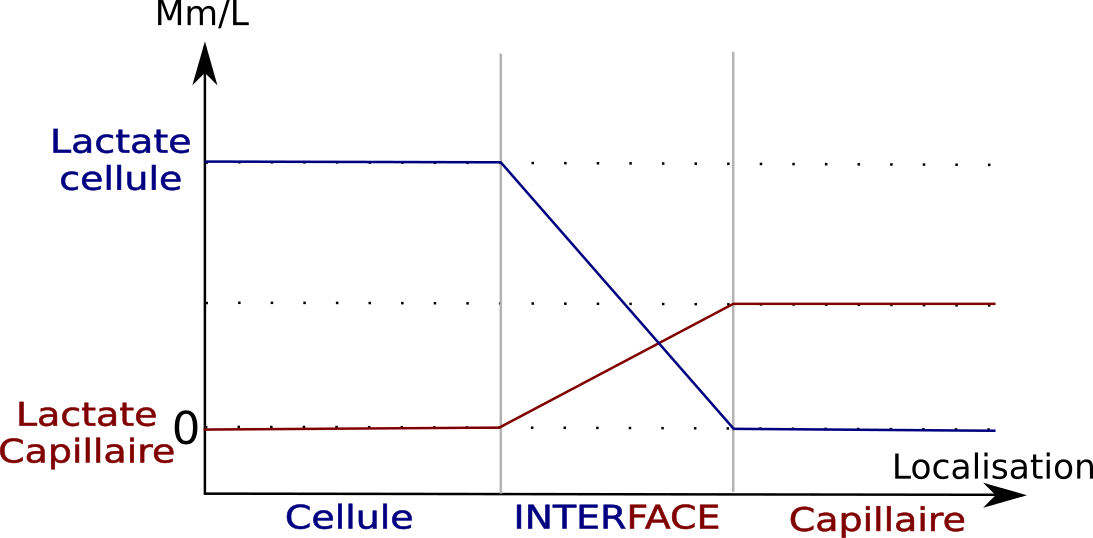
\includegraphics[width=1\textwidth]{dessinD3.png}
\subcaption{Concentrations à l'interface.}
\end{minipage}
\caption{Schéma des modèles mis en place dans cet axe pour le suivi des flux énergétiques en dimension supérieur. (a) Schéma du système de Réaction-Diffusion avec conditions de Neumann, (b) Schéma du systèmes avec des interfaces complexes pouvant préserver le flux , (c) Autre coupe de l'interface proposée par le système complexe. }\label{Lac2}
\end{figure}

\textbf{Communications liées }: Six publications, douze communications orales (dont trois internationales), cinq communications avec support (poster et E-poster).

\newpage
\item[\color{MagSombre}$\bullet$] \textbf{\color{MagSombre}Post-doctorat sous la codirection d'Alain Miranville et Rémy Guillevin, CHU de Poitiers, Laboratoire commun I3M (CNRS-UP-CHU-SIEMENS), Laboratoire de Mathématiques et Applications (LMA, UMR 7348), équipe DACTIM-MIS, 2019-2020.} Mes recherches post-doctorales se concentrent autour de trois axes en continuité de mes recherches doctorales.
\begin{itemize}
\item[$\triangleright$]\textit{Axe 1. Continuité des travaux effectués durant mon doctorat} sur le lactate, le cycle de Krebs et le cycle glutamate dans des conditions pathologiques comme la présence d'une tumeur. Les questions posées ici sont en particulier axées sur, 
\begin{itemize}
\item les interactions entre le cycle de Krebs et le cycle glutamate et aux dérives que cela peut entrainer lors de l'apparition de pathologies mais également les possibilités thérapeutiques qui en découlent \cite{maus2017, stobart2013, kreft2012}. Ces deux cycles ont tous les deux été étudiés durant ma thèse et il semble aujourd'hui important de s'intéresser aux manières dont ils interagissent. Ce modèle est basé sur un système d'EDO entre un neurone et un astrocyte. Ces recherches sont en collaboration avec Nicolas Bourmeyster, laboratoire STIM, ERL CNRS 7003 et Luc Pellerin, laboratoire  Ischémie Reperfusion en Transplantation d’Organes Mécanismes et Innovations Thérapeutiques (IRTOMIT), Inserm U1082.
\item la collecte et le traitement de concentrations en lactate relevées par SRM pour le suivi de patients après la résection d'un gliome. Ces données permettraient de faire évoluer les systèmes proposés durant ma thèse vers des modèles à effets mixtes patient dépendants. Ces résultats pourraient ensuite être utilisés dans la description, la compréhension et l'interprétation de cartes métaboliques fournies par la SRM pour le suivi des patients en routine clinique. Ces recherches sont en collaboration avec Carole Guillevin et Mathieu Naudin, ingénieurs de recherche au CHU de Poitiers, laboratoire commun I3M, laboratoire LMA UMR 7348, équipe DACTIM-MIS.
\end{itemize}
\item[$\triangleright$]\textit{Axe 2. Modélisation des flux calciques.} Les transporteurs ioniques de la biomembrane se trouvent comme les récepteurs à l'interface entre le milieu intracellulaire et le milieu extracellulaire. Ils participent de façon importante à la transmission et à l'intégration de signaux, et donc d'informations, extracellulaires qui proviennent par exemple du microenvironnement tumoral et du stroma. Dans les neurones adultes, et dans les cellules de glioblastomes, ces signaux sont convertis en grande partie par l'activation d'une enzyme qui va générer un signal calcique intracellulaire \cite{Domenichini2018, Terrie2019}. Ce signal est dû à plusieurs mécanismes de gestion des flux calciques. Les plus importants sont : la libération de calcium des réserves présentes dans le réticulum endoplasmique à travers le récepteur à l'inositol trisphosphate (IP$\text{3}$)), l'entrée de calcium depuis le milieu extracellulaire à travers les canaux ioniques Orai1 et TRPC activés par STIM1, la recapture du calcium dans les réserves du réticulum endoplasmique via la pompe calcique SERCA ou, enfin, la sortie du calcium cellulaire dans le mileiu extracellulaire via la pompe calcique PMCA, ou l'échangeur Na$^+$/C$\text{a}^{2^+}$ (voir Figure \ref{Calcium}).  L'augmentation transitoire de la concentration en ion calcium libre dans le cytoplasme active de nombreux processus, impliqués dans la prolifération, l'autorenouvèlement et la migration de cellules dans le cerveau. Nous cherchons à modéliser cette dynamique calcique intracellulaire fondamentale aux fonctions des cellules du cerveau, et qui peut être modifiée dans des cellules cancéreuses de type souche \cite{Terrie2019} grâce à un système de trois EDOs possédant de nombreux termes non linéaires. En particulier, nous cherchons à expliquer de manière mécanique les oscillations calciques observées lors de la majorité des expériences. Nous souhaitons aussi expliquer le fonctionnement de pompes possédant de nombreux paramètres, des valeurs de fonctionnement optimal et des boucles de rétroaction. Ces recherches sont en collaboration avec Bruno Constantin, laboratoire STIM, ERL CNRS 7003.

 \begin{figure}[!htbp]
\centering
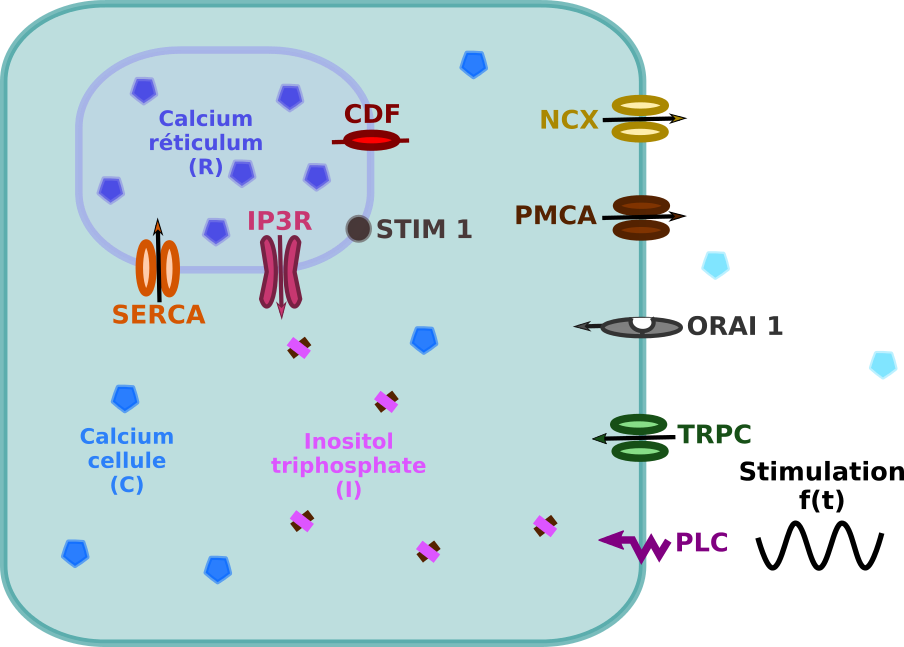
\includegraphics[width=0.6\textwidth]{calcium.png}
\caption{Schéma du modèle mis en place pour l'étude des flux en calcium à travers des transporteurs de mécaniques différentes dans une cellule.}\label{Calcium}
\end{figure}

\item[$\triangleright$]\textit{Axe 3. Etude du profil métabolique suivant un accident vasculaire cérébral (AVC)}. Les patients victimes d'un AVC de moins de 6h pour lesquels une zone du territoire cérébrale moyen a été lésée en oxygène bénéficient à leur admission d'une thrombectomie intravasculaire. Ainsi, on débouche l’artère cérébrale responsable de l’infarctus afin de rétablir la circulation sanguine et donc l'apport en oxygène. Dans les 24h qui suivent ce geste, ils font l'objet d'une exploration IRM multiparamétrique dont une finalité est d'établir un profil métabolique avec des valeurs d'intérêt comme les concentrations de NAA, créatine, choline ou lactate \cite{bruhn1989,parsons2000}. De plus, à 3mois, un score clinique est établi par les neurologues qui permet de quantifier le niveau de handicap distinguant plusieurs groupes pour ces mêmes patients. Le but de cet axe est de définir si des corrélations existent entre ces profils métaboliques et le devenir clinique, de mettre en évidence de possibles paramètres prédictifs et de construire un modèle prédictif en fonction. On aimerait aussi comparer le profil métabolique de ces patients à celui de sujets sains. Ces recherches sont en collaboration avec Guillaume Herpe, chef clinique et doctorant, laboratoire LMA, UMR 7348 et impliquent un stagiaire en M1 de mathématiques, Clément~Giraud. 
\end{itemize}
\textbf{Communications liées }: Un chapitre d'ouvrage en cours $\left[ \text{C1} \right]$, deux communications orales.\\

Les résultats des travaux résumés se satellisent autour des axes de recherche impliqués.
\begin{itemize}
\item \textbf{Mathématiques} : mise en place de modèles adaptés, études statistiques préliminaires, étude mathématique de systèmes d'EDO ou EDP, avec ou sans effet lent-rapide, avec ou sans retard. Ces études comprennent existence, unicité et bornes pour les solutions, étude des états d'équilibre et simulations,
\item\textbf{ Biologie }: description de l'action de pompes ioniques de type symport et modélisation des flux qui en découlent. Analyse des interactions entre différents types de substrats,
\item \textbf{Imagerie} : développement d'outils pour l'optimisation des données issues de la SRM à des fins descriptives et prédictives,
\item \textbf{Médecine} : mise en avant de la sensibilité de certaines dynamiques en substrat pouvant être utilisées à des fins thérapeutiques. Suggestion de la prise en compte possible des concentrations en substrats dans la définition du grade d'une tumeur.
\end{itemize}

\vfill

\item[\color{MagSombre}$\bullet$] {\color{MagSombre}\textbf{Activité liée à la Recherche.}}
\begin{itemize}
\item[$\triangleright$] Mise en place d'un projet de recherche commun avec les départements de mathématiques de Pavie et de Milan (Italie), 4 présentations dans 3 laboratoires différents et durant un workshop entre 2018 et 2019, obtention des bourses du Laboratoire International Associé LYSM AMU CNRS ECM INdAM et de l'European Campus of City-Universities (EC2U), interviews pour le soutien de l'EC2U,
\item[$\triangleright$] Mise en place d'un projet de recherche avec le laboratoire de Signalisation et Transports Ioniques Membranaires (STIM, ERL CNRS 7003), CNRS ERL 7003 - EA 7349, équipe Canaux Calciques et Connexines dans les Cellules Souches (4CS),
\item[$\triangleright$] Obtention de deux bourses du GDR Mamovie (Sept. 2017, Nov. 2018) et du prix Delattre au 37ème Colloque de la Société Francophone de Biologie Théorique (SFBT, Juin 2017).
\item[$\triangleright$] Participation à des écoles d'été,
\begin{itemize}
\item Sept. 2019, Ecole d'été internationale : Mathematical Biology on the Mediterranean Conference, University of Aegean, Samos (Grèce),
\item Juil. 2018, \textmd{Ecole d'été CEMRACS : Numerical and mathematical modeling for biological and medical applications: deterministic, probabilistic and statistical descriptions}, Centre International de Rencontres Mathématiques (CIRM), Marseille,
\item Dec. 2017, \textmd{Ecole d'hiver: Méthodes Déterministes et Stochastiques en Neurosciences}, Centre International de Mathématiques et d'Informatique (CIMI), Toulouse.
\end{itemize}
\item[$\triangleright$] Communications orales lors de manifestations doctorales, 
\begin{itemize}
\item Fev. 2019, \emph{Quand les mathématiques usent d'opérations contre les gliomes.} Séminaire des doctorants de l'école doctorale SISMI, Poitiers, 
\item Oct. 2018, \emph{What about nutrient kinetic in a (gliomatous) brain ?} Conférencière lors du séminaire des doctorants de LAMFA d'Amiens,
\item Mars 2018, \emph{Dynamique des substrats dans le cerveau atteint d'un gliome.} Journées thématiques de l'école doctorale Bio-Santé, Cussac.
\end{itemize}

\end{itemize}
\end{itemize}
\vfill

\newpage
\section{Publications \& Communications}\label{C}
\begin{itemize}
\item[\color{MagSombre}$\bullet$] \textbf{\color{MagSombre} Communications écrites en préparation}
\begin{enumerate}[label={[C\arabic*]}]
\item \hypertarget{C1} Perrillat-Mercerot A., Miranville A., Bourmeyster N. and Guillevin R. \textit{Mathematics as a paradigm for cerebral studies}, \textbf{En préparation}.
\item \hypertarget{C1} Perrillat-Mercerot A., Miranville A., Agosti A., Grasselli M., Rocca E., Ciarletta P. and Guillevin R. \textit{PDE system with irregular bounds conditions for lactate kinetics}, \textbf{En préparation}.
\end{enumerate}

\item[\color{MagSombre}$\bullet$] \textbf{\color{MagSombre} Publications dans des revues internationales à comité de lecture (celles soulignées seront fournies en cas d'audition)}
\begin{enumerate}[label={[C\arabic*]},resume]
\item  \hypertarget{C2} Perrillat-Mercerot A., Guillevin C., Miranville A. and Guillevin R. (2019). \textit{Using mathematics in MRI data management for glioma assesment}, Journal of Neuroradiology.
\item \hypertarget{C3} Perrillat-Mercerot A., Miranville A., Bourmeyster B., Guillevin C.,  Naudin M., and Guillevin R. (2019). \textit{What mathematical models can or cannot do in glioma description and understading},Discrete \& Continuous Dynamical Systems-S.
\item \hypertarget{C4}{Perrillat-Mercerot A., Bourmeyster N., Guillevin C., Miranville A. and Guillevin R. (2019). \textit{Analyse of a mathematical model for the glutamate/glutamine cycle}. Bulletin of Mathematical Biology, 1-20.}
  \item \hypertarget{C5}{Perrillat-Merceot A., Bourmeyster N., Guillevin C., Miranville, A., and Guillevin, R. (2019). \textit{Mathematical Modeling of Substrates Fluxes and Tumor Growth in the Brain}. Acta biotheoretica, 1-27} 
  \item \uline{Guillevin C., Guillevin R., Miranville A., and Perrillat-Mercerot A. (2018). Analysis of a mathematical model for brain lactate kinetics. Mathematical Biosciences \& Engineering, 15(5), 1225-1242. Ordre alphabétique.}
     \item \uline{Helal, M., Igel-Egalon, A., Lakmeche, A., Mazzocco, P., Perrillat-Mercerot, A., Pujo-Menjouet, L., Rezaei H. \& Tine, L. M. (2018). Stability analysis of a steady state of a model describing Alzheimer's disease and interactions with prion proteins. Journal of Mathematical Biology, 1-25. Ordre alphabétique.} 
    \item \uline{Guillevin R., Miranville A. and Perrillat-Mercerot A. (2017). On a reaction-diffusion system associated with brain lactate kinetics Electronic Journal of Differential Equations, (23), 1-16. Ordre alphabétique.}
\end{enumerate}
\item[\color{MagSombre}$\bullet$] \textbf{\color{MagSombre}Communications orales nationales.}
\begin{itemize}
\item[$\triangleright$] Perrillat-Mercerot A., \textit{Utilisation des Mathématiques dans l'imagerie médicale, application à l'étude des tumeurs du cerveau}, Table ronde pour les 80ans du CNRS - pôle santé, Poitiers, Dec. 2019.
\item[$\triangleright$] Perrillat-Mercerot A., \textit{Modèles en neuro-oncologie}, Workshop Oncosphère Nouvelle-Aquitaine, Angoulême, Dec. 2019.
\item[$\triangleright$] Perrillat-Mercerot A., \textit{Approche des fux de lactate cérébral, du 1D au 3D}, 39$^{\text{ème}}$ Colloque de la Société Francophone de Biologie Théorique (SFBT), Poitiers, Juin 2019.
\item[$\triangleright$] Perrillat-Mercerot A., \textit{Mathématiques et gliome, une histoire d'opérations.}, 39$^{\text{ème}}$ Colloque de la Société Francophone de Biologie Théorique (SFBT), Poitiers, Juin 2019.
\item[$\triangleright$] Perrillat-Mercerot A., \textit{Quand les mathématiques usent d'opérations contre les gliomes}, Congrès 2019 de l'Association des Neuro-Oncologies d'Expression Française (ANOCEF), Poitiers, Juin 2019.
\item[$\triangleright$] Perrillat-Mercerot A., \textit{How MRI and mathematics can get together}, Invitée par l'Université de Pavia, Pavia (Italie), Mai 2019.
\item[$\triangleright$] Perrillat-Mercerot A., \textit{Quand les mathématiques usentd'opérations contre les gliomes} Présentation orale lors du Forum Jeunes Mathématiciennes et Mathématiciens, Mathématiques et Sciences du Vivant, Orléans, Nov. 2018.
\item[$\triangleright$] Perrillat-Mercerot A., \textit{What about nutrient kinetic in a (gliomatous) brain ?} Invitée par Polytecnico di Milano pour une collaboration entre laboratoires, Milano (Italie), Nov. 2018.
\item[$\triangleright$] Perrillat-Mercerot A., \textit{What about nutrient kinetic in a (gliomatous) brain ?} Invitée par l'Universita di Pavia pour une collaboration entre laboratoires, Pavia (Italie), Nov. 2018.
\item[$\triangleright$] Perrillat-Mercerot A., \textit{Un modèle pour l'étude de la croissance tumorale.} Journée maths et cancer, Poitiers, Sept. 2017,
\item[$\triangleright$] Perrillat-Mercerot A., \textit{Modèle réduit pour la cinétique du lactate.} 37$^{\text{ème}}$ Colloque de la Société Francophone de Biologie Théorique (SFBT), Poitiers, Juin 2017. 
\end{itemize}

\item[\color{MagSombre}$\bullet$] \textbf{\color{MagSombre}Communications orales internationales.}
\begin{itemize}
\item[$\triangleright$] Perrillat-Mercerot A.,\textit{Investigation on complex nutrient 
fluxes}, International Workshop Mathematical Biology on the Mediterranean Conference (MBMC), Samos (Grèce), Sept. 2019.
\item[$\triangleright$] Perrillat-Mercerot A., \textit{Substrate fluxes between cells and capillaries}, Workshop Recent advances in Phase-Field modeling: from Engineering to Biology, Pavia (Italie), Mai 2019.
\item[$\triangleright$]  Perrillat-Mercerot A., \textit{What about lactate kinetic in a (gliomatous) brain ?}, conférencière invitée à la session spéciale Recent Advances in Mathematical Biology, Ecology, Epi-demiology, and Oncology organisée par Sophia Jang, Hsiu-Chuan Wei, Ting-Hui Yang, Jui-Ling Yu et Alain Miranville, The 12th AIMS Conference on Dynamical Systems, Differential Equations and Applications, Taipei (Taiwan), Juil. 2018.
\end{itemize}
\item[\color{MagSombre}$\bullet$] \textbf{\color{MagSombre}Communications avec support (poster \& E-poster).} \begin{itemize}
\item[$\triangleright$] Perrillat-Mercerot A., \uline{Bourmeyster N.}, Miranville A., Guillevin R. and  Guillevin C. \textit{Let's make maths about lactate in the brain}, 23rd ESN Biennial Meeting - 7th Conference on Molecular Mechanisms of Regulation in the Nervous System, Milan, Sept. 2019.
\item[$\triangleright$] \uline{Perrillat-Mercerot A.}, Guillevin C., Guillevin R. and Miranville A. \textit{Modélisation mathématique des flux de glutamate intracérébraux
intégrant les données RMN spectroscopiques.} 45$^\text{éme}$ congrès de la Société Française de Neuroradiologie (SFNR), Paris, Mars 2018.
\item[$\triangleright$]   \uline{Perrillat-Mercerot A.}, Guillevin C., Guillevin R. and Miranville A. \textit{Data Analysis and Computation Though Imaging and Modeling - Maths Image Santé.} Journées Francophones de radiologie - Village des innovations, Paris, Sept. 2017.
\item[$\triangleright$] \uline{Perrillat-Mercerot A.}, Guillevin C., Guillevin R. and Miranville A. \textit{Un modèle pour l'étude de la croissance tumorale.} Journée maths et cancer, Poitiers, Sept. 2017.
\item[$\triangleright$] \uline{Perrillat-Mercerot A.}, Guillevin C., Guillevin R. and Miranville A.  \textit{Dynamique des substrats énergétiques dans le cerveau atteint d'un gliome.} Poster pour le congrès 2017 de l'Association des Neuro-Oncologies d'Expression Française (ANOCEF), Nancy, Juin 2017.
\end{itemize}
\end{itemize}

\newpage
\section{Projet de Recherche \& d'Enseignement}

Cette partie a été adaptée pour chaque candidature, je n'en propose ici qu'un très bref résumé. Merci de me contacter pour toute information ou proposition.\\

Mon projet de recherche se découpe suivant des problématiques biomathématiques diverses. Mon projet d'enseignement est stimulé par des motivations pluridisciplinaires, numériques et d'accessibilité.
Motivée et dynamique, je reste naturellement à l'écoute des autres projets et des besoins du laboratoire, espérant pouvoir construire des démarches pertinentes et adaptées pour répondre aux problématiques soulevées. Déterminée à être rapidement opérationnelle au sein d'une université innovante, continuer mes travaux dans vos équipes pluridisciplaines et actives me permettrait aussi d'élargir mon domaine de compétences et d'initier de nouveaux projets communs. Je reste à votre disposition pour de plus amples informations, espérant pouvoir vous présenter de vive voix ma motivation et mon dynamisme.\\
 
%\nocite{*}
\addtocounter{section}{1}
\addcontentsline{toc}{section}{7\hspace{0.4cm}Références} 
\bibliographystyle{siam-fr}
\bibliography{dossier}

\vfill

\section{Annexes}
 \begin{itemize}
\item[\color{MagSombre}$\bullet$] \textbf{\color{MagSombre}Liste des documents joints à la candidature.}
 \begin{itemize}
 \item[$\triangleright$] Copie du diplôme de doctorat en mathématiques obtenu en 2019,
 \item[$\triangleright$] Copie des rapports de pré-soutenance rédigés par Olivier Saut et Jean-Noël Vallée,
\item[$\triangleright$] Copie du rapport de soutenance de thèse datée du 22 octobre 2019,
\item[$\triangleright$] Lettres de recommandation de docteurs en mathématiques : Alain Miranville, Laurent Pujo-Menjouet et Jacques Demongeot,
\item[$\triangleright$] Lettres de recommandation de docteurs en sciences du vivant : Rémy Guillevin (radiologie et imagerie médicale), Nicolas Bourmeyster (biochimie et biologie moléculaire), Jacques Demongeot (biostatistiques, informatique médicale et technologies de communication), 
\item[$\triangleright$] Lettre de recommandation pour l'enseignement : Laurence Di Poi, PRAG. 
 \end{itemize} 
 \end{itemize} 
 
 \vfill
 ~
 
\end{document}
